% Chapter Template

\chapter{PANACM NANOPARTICULAS} % Main chapter title

\label{C4} % Change X to a consecutive number; for referencing this chapter elsewhere, use \ref{ChapterX}

\lhead{Capítulo 4. \emph{PANACM NANOPARTICULAS}} % Change X to a consecutive number; this is for the header on each page - perhaps a shortened title

%----------------------------------------------------------------------------------------
%	SECTION 1
%----------------------------------------------------------------------------------------

\section{INTRODUCTION}

ABSTRACT DEL PAPER

La plasticidad en vidrios metálicos glasses (en inglés bulk metallic glasses o BMGs) es en general controlada inicialmente por zonas de transformación de tensión cortante (en inglés shear transformation zones o STZs), las cuales se expanden para formar bandas de corte (en inglés shear bands o SBs) a través del material. Para contorlar y por consiguiente mejorar la dinámica de la plasticidad, la composición de los vidrios metálicos ha sido modificada de diferentes maneras.

Particularmente, la inclusión de nanopartículas cristalinas provee obstáculos a la propagación y crecimiento de SBs, que frecuentemente se nuclean (se originan?) en la interface entre el BMG y la nanopartícula. Ésto se traduce en una deformación más reducida y homogénea en régimen plástico. Sin embargo, para asegurar efectos perdurables, las inclusiones deberían ser estables en el tiempo, es decir, no difundir en el material amorfo circundante perdiendo así la transición nítida entre cristal y amorfo.

Se muestran resultados para inclusiones de cobre cristalino con estructura de cubo centrada en las caras (FCC). Aunque no nos enfocamos en los efectos del tamaño de las inclusiones como otros estudios, analizamos la estabilidad de las nanopartículas a diferentes temperaturas. Durante la deformación mecánica de la muestra de un BMG con inclusiones bajo esfuerzo de tracción uniaxial, analizamos los polyedros de Voronoi y la distribución de esfuerzo y deformación cortante para estudiar el papel de la inclusión en las propiedades mecánicas de este material compuesto.

INTRODUCCION DEL PAPER

Bulk Metallic Glasses (BMG) are known for their outstanding mechanical properties such as elasticity, strength and hardness, and because of this they are matter of deep research. However, the tendency to massively collapse initially formed shear transformation zones (STZs) into a single shear band (SB) and thus failing catastrophically, restricts their plasticity and their applications \cite{cao09, xiao12}.

It is of much interest the modification of their composition so as to enhance these restraints \cite{albe13, adibi13, adibi14}. In particular, the inclusion of crystalline nanoparticles promote the nucleation of STZs and act as an impediment to the propagation of SBs \cite{albe13}. As a result, a reduced and more homogeneous deformation in the plastic regime is obtained.

After analyzing constitutive parameters of the Cu$_{46}$Zr$_{54}$ metallic glass used as matrix in this work \cite{ardiani12}, we now focus on the stability at different temperatures of spherical face-centered cubic (FCC) Cu inclusions using Molecular Dynamics (MD) simulations. Voronoi polyheadra, shear stress and shear strain are analyzed in the deformation process under uniaxial strain of the BMG in order to get a better understanding of the role of the inclusion in the mechanical properties of this composite material.

\section{SIMULATION DETAILS}

%We use the LAMMPS software package \cite{plimpton95} for running all the simulations, which is free and open source.

%The original sample is a Cu$_{46}$Zr$_{54}$ metallic glass with 160k atoms, obtained with a quenching rate of 10$^{12}$ K/s with an experimental glass transition temperature (\textit{T$_{g}$}) of 696 K, and it has already been described in \cite{arman10}.
%An embedded atom method (EAM) potential is adopted \cite{daw84}, used previously in other works on BMGs \cite{cao09, arman10, shimizu07, cheng09, cheng11, wang12}. Periodic boundary conditions are used in all directions, to mimic high strain rate loading conditions.

Analizamos inclusiones esféricas de cobre FCC. Una región de 2 nm de radio es eliminada de la muestra en una posición central, la cual fue luego llenada con la red cristalina correspondiente, es decir, una red cristalina FCC con una constante de red de 0.3615 nm. Luego de creados los átomos de Cu en la región esférica, la configuración fue minimizada, luego equilibrada a presión cero por algunos ps, luego calentada (o enfriada) para alcanzar la temperatura final deseada (\textit{T$_{f}$}) durante 4 ps y fue finalmente RECOCIDA(?) TEMPLADA(?) a \textit{T$_{f}$} por 1 ns.

En esta sección nos centramos en la estabilidad de las nanopartículas a diferentes temperaturas, aunque mostraos algunos casos de sometimiento a tracción y compresión uniaxial. Una velocidad de deformación homogénea de 10$^{9}$/s es aplicada. La Difusividad en todos los casos se calcula ajustando los desplazamientos cuadráticos medios (en inglés mean squared displacements o MSD), $\langle r^{2}\rangle$, obtenidos de LAMMPS.

\section{RESULTS}

\subsection{Inclusion Stability}

En esta sección analizamos la estabilidad de nanopartículas a diferentes temperaturas, hasta temperaturas cercanas a la transición vítrea.

La información obtenida de los MSD para los átomos de la inclusión se obtienen de simulaciones a diferentes temperaturas. Como podemos ver en la Figura \ref{figure:msd_Cu} \subref{figure:msd10_400}, luego de un transitorio inicial, los MSD se vuelven casi costantes, conduciendo a una difusividad cercana a cero, como es de esperar para una inclusión solida estable.

Esto indicaría que las inclusiones son de hecho estables en condiciones de operación normal para BMGs. Sin embargo, las simulaciones de MD cubren típicamente un corto periodo de tiempo de sólo algunos ns, y nos centramos ahora en temperaturas más elevadas para una mejor evaluación de la estabilidad de la nanopartícula.

Usamos entonces la información para T $ \geq 500$ K (Figura \ref{figure:msd_Cu} \subref{figure:msd500_800}), y obtenemos difusividades que se muestran en la Tabla \ref{table:FCC_Diff_Fit_Restults}, usando la ecuación de Einstein $\langle r^{2}\rangle = 6Dt$, para tiempos superiores a 0.6 ns, cuando hay una pendiente estable.

Estos resultados representan una media de todas los átomos de la nanopartícula, pero podrían existir grandes direfencias entre los átomos del núcleo y la superficie de la inclusión. Es por ésto que calculamos los MSD de los átomos de Cu en una región de coróna esférica de un espesor de 0.8 nm y radio interno de 1.2 nm. Puede verse en la Figura \ref{figure:FCCdiff_shell_comp} que, luego de un transitorio de unos 0.6 ns, las pendientes de los MSD son prácticamente iguales para la corona y la nanopartícula en su totalidad, y podemos usar las difusividades de la Tabla \ref{table:FCC_Diff_Fit_Restults}.

Las Difusividades para T $ \geq 500$ K son ajustadas para tener correspondencia con la ecuación \ref{equation:diff_Fit}, donde $k_{B}$ es la constante de Boltzmann, $\Delta E$ es la energía de activación para difusión, y $D_{0}$ da la escala de difusividad. La regresión resultante aparece en la Tabla \ref{table:FCC_Diff_VS_T_Fit_Restults} y son mostrados gráficamente en la Figura \ref{figure:FCC_diff_vs_T}.

\begin{figure}[htp]
\centering
\subfloat[Lower temperatures]{
	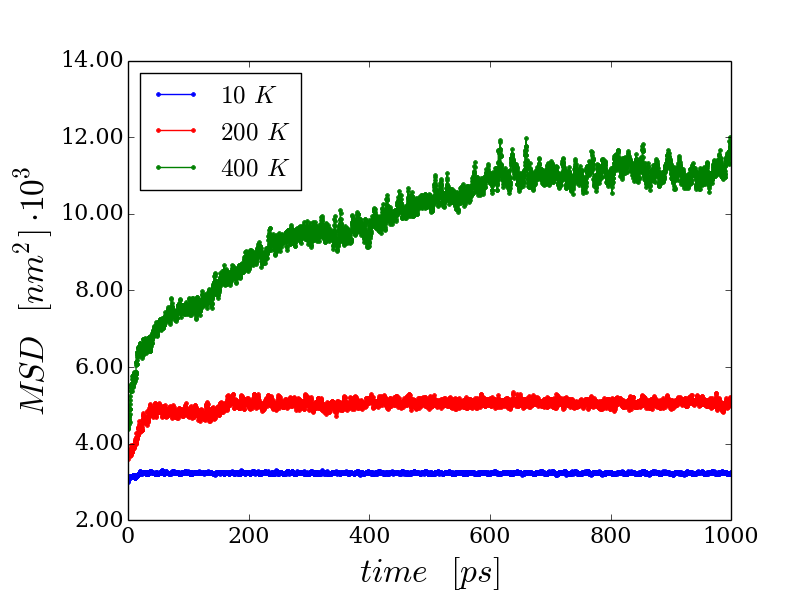
\includegraphics[width=10cm]{Cap_4/msd10_400_FCC.png}
	\label{figure:msd10_400}}
\\
\subfloat[Higher temperatures]{
	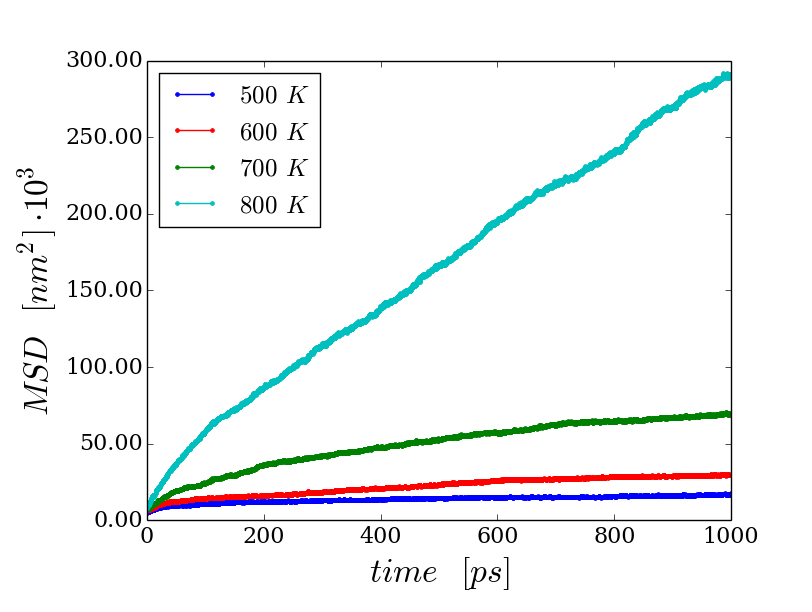
\includegraphics[width=10cm]{Cap_4/msd500_800_FCC.png}
	\label{figure:msd500_800}}
\caption{MSD para inlusión de Cu FCC a diferentes temperaturas}
\label{figure:msd_Cu}
\end{figure}

\begin{table}[htp]
\caption{Resultados del ajuste de la Difusividad}
\begin{center}
\begin{tabular}{*{3}{c}}
\hline
T [$K$] & D [$\frac{nm^{2}}{ps}$] & R$^{2}$ \\
\hline
500 & $8,490\cdot 10^{-7}$ & 0,8306 \\
\hline
600 & $1,508\cdot 10^{-6}$ & 0,9253 \\
\hline
700 & $4,699\cdot 10^{-6}$ & 0,9357 \\
\hline
800 & $4,149\cdot 10^{-5}$ & 0,9935 \\
\hline
\end{tabular}
\end{center}
\label{table:FCC_Diff_Fit_Restults}
\end{table}

\begin{figure}[htp]
\centering
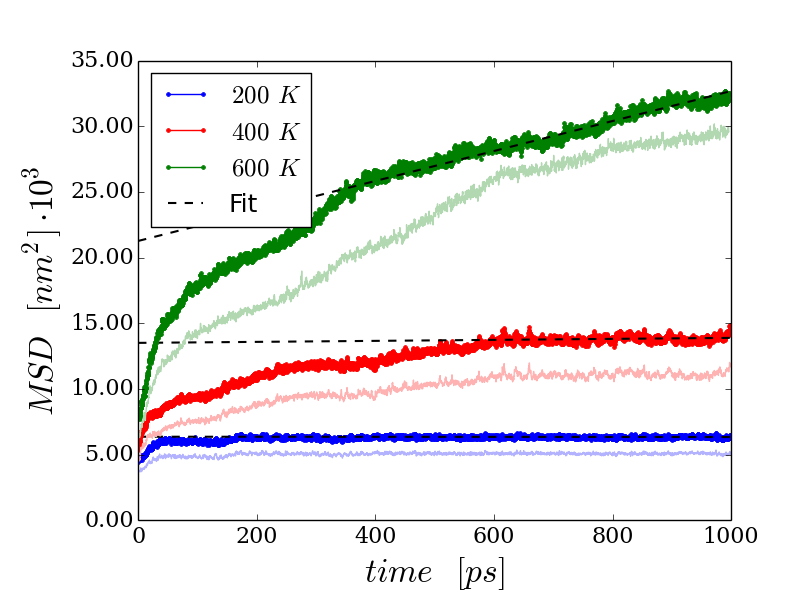
\includegraphics[width=10cm]{Cap_4/FCCdiff_shell_comp.png}
\caption{MSD de la corona esférica y para la nanopartícula completa (color más claro)}
\label{figure:FCCdiff_shell_comp}
\end{figure}

\begin{eqnarray}
D = D_{0}\cdot \mathrm{e}^{\frac{-\Delta E}{k_{B} T}}
\label{equation:diff_Fit}
\end{eqnarray}

\begin{figure}[htp]
\centering
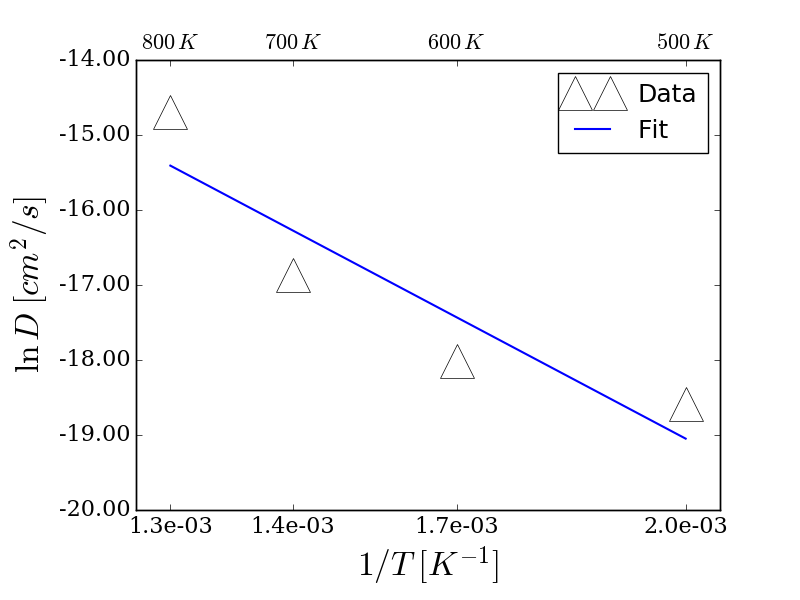
\includegraphics[width=10cm]{Cap_4/FCCDiff_vs_temp_fit.png}
\caption{Difusividad en función de la temperatura}
\label{figure:FCC_diff_vs_T}
\end{figure}

\begin{table}[htp]
\caption{Resultados del ajuste de la Difusividad con respecto a la temperatura}
\begin{center}
\begin{tabular}{*{2}{c}}
\hline
Activation energy [$eV$]& $-0,4182$ \\
\hline
D$_{0}$ [$\frac{nm^{2}}{ps}$] & $8,771\times 10^{-3}$\\
\hline
R$^{2}$ & 0,8399 \\
\hline
\end{tabular}
\end{center}
\label{table:FCC_Diff_VS_T_Fit_Restults}
\end{table}

Como fué señalado en \cite{albe13}, el núcleo de las inclusiones se ve reducido porque los átomos más externos tienden a volverse amorfos. Este efecto se incrementa con la temperatura, como era de esperarse, cuando la difusión atómica es mayor.

\subsection{Uniaxial Loading}

En esta sección, presentamos resultados sobre el sometimiento a esfuerzos uniaxiales del BMG que contiene una nanopartícula, como se describió anteriormente.

Las Figuras \ref{figure:fcc_vm_tension} y \ref{figure:fcc_vm_compression} muestran la muestra bajo esfuerzos uniaxiales de tracción y compresión para T = 10 K y T = 400 K. Consideramos estas dos temperaturas como representativas de un régimen de baja y otro de alta temperatura, pero para temperaturas para las que la difusividad es pequeña y la nanopartícula estable.

La apariencia de las curvas esfuerzo-deformación sigue un comportamiento esperado observado para el material sin ningúna inclusión. La pequeña inclusión no afecta el régimen elástico, y a una temperatura elevada, el ABLANDAMIENTO(?) del BMG tampoco es afectado, tanto para tracción como para compresión. El esfuerzo máximo se ve decrementado ligeramente por la nanopartícula a bajas temperaturas. El esfuerzo de ?? a grandes deformaciones no se ve modificado por la inclusión bajo compresión. Por otro lado, la nucleación de un poro bajo tracción, indicada por la repentina caída de esfuerzo, se ve algo retrasada por la inclusión, permitiendo alrededor de un 1\% de deformación adicional de la muestra. Ésto podría explicarse por alguna relajación y disipación ocurriendo en la frontera entre la nanopartícula y el BMG, pero un estudio más detallado debería realizarse para aclarar la situación.

Bajo tracción (Figura \ref{figure:fcc_vm_tension}), incluso si al parecer la deformación atómica cortante parece concentrarse en la frontera de la inclusión ubicada en la zona central de la muestra como se ve en la Figura \ref{figure:fcc_tension_bmg_10K}, una deformación plástica homogénea está presente, con nucleacion abundante de STZs, probablemente debido a la alta velocidad de deformación y alta velocidad de templado de la muestra, llevando a la nucleación de un poro en una zona distinta a la frontera entre el BMG y la nanopartícula. Bajo compresión a baja temperatura, también encontramos STZs, como vemos en la Figura \ref{figure:fcc_compression_bmg_10K}.

Como algunos poliedros de Voronoi son considerados ser estructuras más resistentes al esfuerzo conrtante, particularmente las agrupaciones de icosaedros \cite{cheng08}, mostramos la evolución de la fracción de icosaedros en la muestra y la comparamos con la muestra de BMG original sin inclusiones y a 10 K. Podemos ver en la figura \ref{figure:fcc_voro_10K} que las fracciones siguen el mismo comportamiento que en la muestra sin nanopartícula. Bajo tracción, la nucleación de un poro da origen a fluctuaciones. Vale la pena notar que estas fluctuaciones corresponden a una deformación más elevada como ya se había mencionado para la curva de esfuerzo-deformación.

\begin{figure}[h!]
\centering
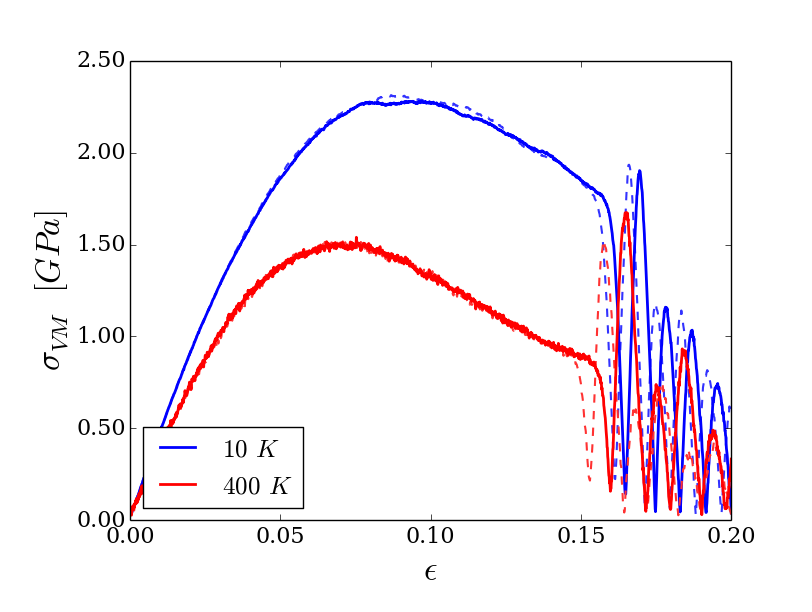
\includegraphics[width=10cm]{Cap_4/vm_vs_strain_tension_MIN.png}
\caption{vonMises stress vs strain for the BMG under uniaxial tension with no inclusion (dotted line) and one inclusion (solid line)}
\label{figure:fcc_vm_tension}
\end{figure}

\begin{figure}[h!]
\centering
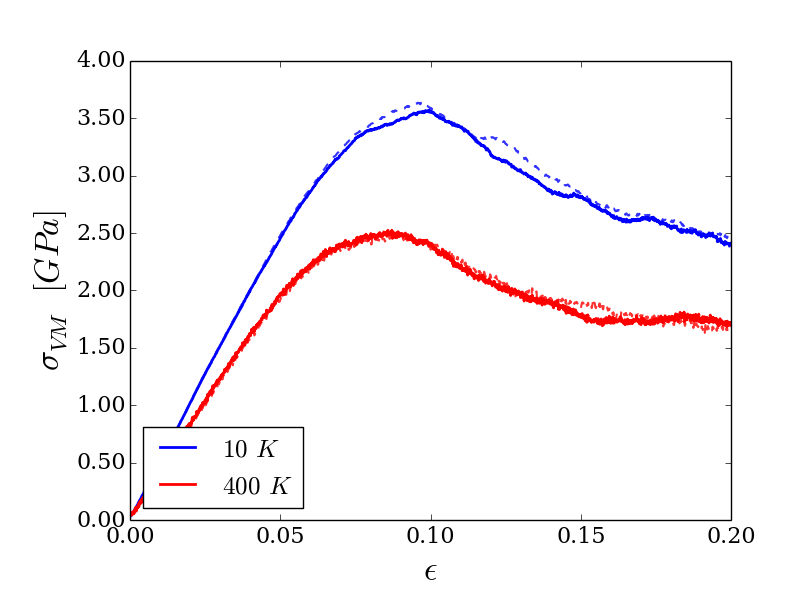
\includegraphics[width=10cm]{Cap_4/vm_vs_strain_compression_MIN.png}
\caption{vonMises stress vs strain for the BMG under uniaxial compression with no inclusion (dotted line) and one inclusion (solid line)}
\label{figure:fcc_vm_compression}
\end{figure}

\begin{figure}[h!]
\centering
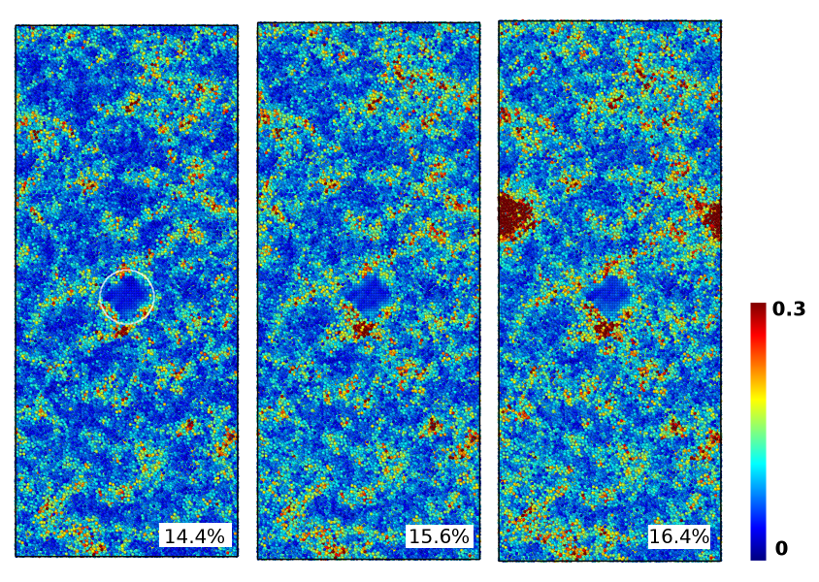
\includegraphics[width=14cm]{Cap_4/FCC_Tension_10K_LOWRES.png}
\caption{Snapshots of sample under tension at selected strains at 10 K (inclusion pointed out in first snapshot). Color represents atomic shear strain.}
\label{figure:fcc_tension_bmg_10K}
\end{figure}

\begin{figure}[h!]
\centering
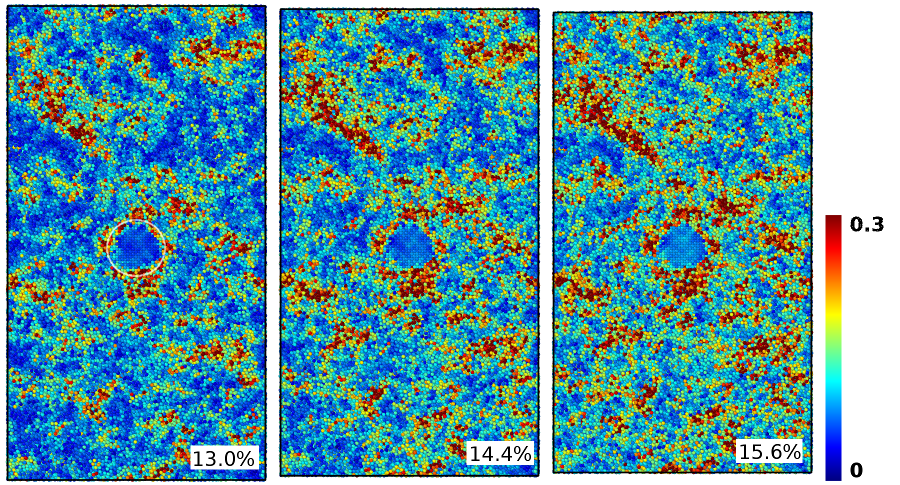
\includegraphics[width=14cm]{Cap_4/FCC_Compression_10K_LOWRES.png}
\caption{Snapshots of sample under compression at selected strains at 10 K (inclusion pointed out in first snapshot). Color represents atomic shear strain.}
\label{figure:fcc_compression_bmg_10K}
\end{figure}

\clearpage

\begin{figure}[h!]
\centering
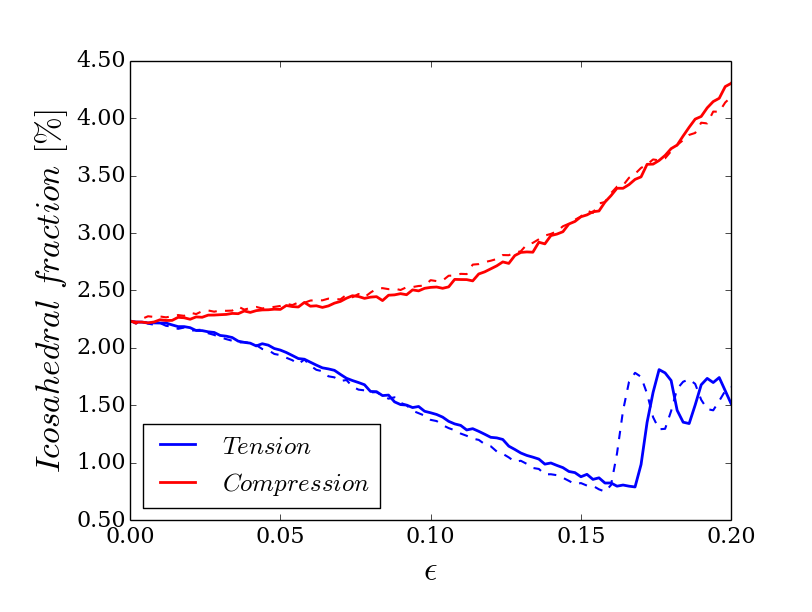
\includegraphics[width=12cm]{Cap_4/FCC_voro_vs_strain_10K_B.png}
\caption{Icosahedral fraction under tension and compression at 10 K. Dotted line represents original sample.}
\label{figure:fcc_voro_10K}
\end{figure}

\section{SUMMARY AND CONCLUSIONS}

Estudiamos un BMG con una nanopartícula cistalina como inclusión. Consideramos un vidio CuZr, y una nanopartícula de Cu pura con un radio de 2 nm. Ésto implica una fracción en volumen que varía desde 1.15\% a 10 K hasta 1.12\% a 800 K como resultado del aumento del volumen inicial de la muestra con la temperatura. Una situación similar fue explorada recientemente po Albe et al. \cite{albe13}. Aquí, nos centramos en los efectos de la temperatura, e inicialmente estudiamos la estabilidad debajo de los 400 K, indicando que la nanopartícula es bastante estable a esas tempearturas. A temperaturas mayores, la difusividad en sólo algunos ns trae consigo la pérdida de una interfaz nítida entre la nanopartícula y la matriz.

En nuestras simulaciones, se aplicaron condiciones de frontera periódicas en tres dimensiones, y la ausencia de superficies libres deja sólo a la nanopartícula como probable concentrador de esfuerzo para pomover la nucleación de STZs, como GERMEN(?) para las bandas de corte, en la interfaz entre la matriz y la nanopartícula. Sin embargo, éste no fue el caso. Las curvas de esfuerzo-deformación son claramente similares al caso sin nanopartícula, a excepción de un retardo en la nucleación de un poro bajo tracción para la muestra con una nanopartícula.

El análisis de Voronoi no muestra diferencias significativas entre las muestras con y sin inclusión de nanopartícula. Un estudio futuro y más detallado es requerido para diferentes modos de carga y temperaturas. Estudios futuros también podrían repetir estos experimentos con inclusiones de CuZr con una estructura cristalina B2, como podemos encontrar en algunas experiencias \cite{wei14, kuo14}.